%%%%%%%%%%%%%%%%%%%%%%%%%%%%%% -*- Mode: Latex -*- %%%%%%%%%%%%%%%%%%%%%%%%%%%%
%% ptr.tex         : 2009 Post Tenure Review
%% Author          : Philip Johnson
%% Created On      : Tue Mar 31 11:16:58 2009
%% Last Modified By: Philip Johnson
%% Last Modified On: Mon Jan  4 13:36:07 2010
%%%%%%%%%%%%%%%%%%%%%%%%%%%%%%%%%%%%%%%%%%%%%%%%%%%%%%%%%%%%%%%%%%%%%%%%%%%%%%%
%%   Copyright (C) 2009 
%%%%%%%%%%%%%%%%%%%%%%%%%%%%%%%%%%%%%%%%%%%%%%%%%%%%%%%%%%%%%%%%%%%%%%%%%%%%%%%
%% 
 
\documentclass[11pt]{article}
\usepackage[final]{graphicx}

%% Make subsubsections numbered and included in ToC
\setcounter{secnumdepth}{3}
\setcounter{tocdepth}{3}

\usepackage{multirow}

%% URLs
\usepackage{url}
\usepackage[colorlinks, bookmarks=true]{hyperref}

%% Define a new 'smallurl' style for the package that will use a smaller font.
\makeatletter
\def\url@smallurlstyle{%
  \@ifundefined{selectfont}{\def\UrlFont{\sf}}{\def\UrlFont{\small\ttfamily}}}
\makeatother
%% Now actually use the newly defined style.
\urlstyle{smallurl}

%% CO2 
\usepackage{xspace}
\newcommand{\COtwo}{CO\ensuremath{_2}\xspace}

%% Make margins less ridiculous
\usepackage{fullpage}

%% Since I'm using the LaTeX Makefile that uses dvips, I need this
%% package to make URLs break nicely
\usepackage{breakurl}

\begin{document}
\title{{\bf Philip M. Johnson \\ 
       Post Tenure Review \\ 
       January 2005 to December 2009}}

\author{Philip M. Johnson \\
      Collaborative Software Development Laboratory \\
      Department of Information and Computer Sciences \\
      University of Hawai'i,  Honolulu, HI 96822 \\
      johnson@hawaii.edu 
}

\maketitle

%\tableofcontents


\section{Research}

My research activities during the past five years involved the following
major projects: the Collaborative Software Development Laboratory (CSDL),
the Hackystat Project, the Renewable Energy and Island Sustainability
Project (REIS), and iSustainability.

\subsection{CSDL}

I established the Collaborative Software Development Laboratory (CSDL) in 1991, shortly after joining the University of Hawaii faculty.  CSDL occupies a suite of offices in the POST Building (Room 307). The goal of CSDL is ``to create a physical, organizational, technological, and intellectual environment conducive to collaborative development of world-class software engineering skills. Through research, education, and technology transfer, we pursue this goal for CSDL members, the University of Hawaii, our affiliates, and the Hawaiian, U.S., and international software research and development communities.''

\paragraph{Students.} Since 2005, I have provided direct research supervision for 6 Ph.D. students, 7 M.S. students, and 4 B.S. students under the auspices of CSDL, as detailed in Figure \ref{fig:students}.

\begin{figure}[ht]
\small
\begin{tabular}{p{2in}p{2in}p{2in}} \hline
Robert Brewer (Ph.D., current) & Pavel Senin (Ph.D., current)  & Shaoxuan Zhang (M.S., 2009) \\
Alexey Olkov (M.S., 2009) & Ka Yee Leung (B.S., 2009) & Qin Zhang (Ph.D., 2007) \\
Hongbing Kou (Ph.D., 2007) & Mike Paulding (M.S, 2006)  & Takuya Yamashita (M.S., 2005) \\
James Wang (B.S., 2005) & Aaron Kagawa (M.S., 2005) & Christoph Lofi (M.S., 2005) \\
Austin Ito (B.S., 2005) & Julie Sakuda (B.S., 2005) & Randy Cox (M.S., unfinished) \\
David Nickles (Ph.D., unfinished) & \multicolumn{2}{l}{Tryggvi Bjorgvinsson (Ph.D., unfinished)}  \\ \hline
\end{tabular} \\ 
\normalsize
\caption{Students in CSDL since 2005}
\label{fig:students}
\end{figure}

\paragraph{Website.} CSDL has an online presence at
\url{http://csdl.ics.hawaii.edu}. In 2008, we redesigned and reimplemented 
the CSDL website over the course of 12 months with the
assistance of Pam Scott, an LIS student.  The Plone-based CSDL website 
now provides extensive information about the lab, including overviews of
29 current and completed research projects, our online tech
report library with 193 publications, 35 current and former CSDL
members, 15 affiliate organizations, and dozens of news items regarding the lab, as
illustrated in Figure \ref{fig:csdl}.

\begin{figure*}[th]
  \center
  \includegraphics[width=\textwidth]{csdl.eps}
  \caption{The CSDL Home Page}
  \label{fig:csdl}
\end{figure*} 

\newpage
\paragraph{Funding.} Figure \ref{fig:funding} summarizes the 14 funding opportunities (3 pending, 6 awarded, 5 declined) that I have pursued since 2005. All of the funding opportunities were extramural, with the sole exception of Renewable Energy and Island Sustainability, which was a University of Hawaii intramural funding competition involving approximately 15 UH faculty. 

\begin{figure}[ht]
\small
\begin{tabular}{p{4.5in}rrr} \hline
{\bf Title, Organization (Year)} & {\bf Role} & {\bf \$ Amount} & {\bf Status} \\
Human Centered Information Integration for the Smart Grid, NSF (2009) & PI
& 381,468 & Pending \\
Renewable Energy and Island Sustainability, NSF (2009) & Sen. Per. & 3,200,000 & Pending \\
Clean Energy and Island Sustainability, DOE (2009) & Sen. Per. & 2,500,000 & Pending \\
Renewable Energy and Island Sustainability, UH (2009) & co-PI & 1,000,000 & Awarded  \\
Empirical Computational Thinking, NSF (2009) & PI & 298,237 & Declined \\
Google Summer of Code, Google (2009) & PI & 25,000 & Awarded \\
Google Summer of Code, Google (2008) & PI & 20,000 & Awarded \\
Hackystat Development Donation, Expedia, Inc. (2008) & PI & 25,000 & Awarded \\
A Science of Design Empirical Testbed, NSF (2007) & PI & 367,672 & Declined \\
Discovery and evaluation of software engineering best practices, NSF (2007) & PI & 371,592 & Declined \\
Hackystat Development Donation, Sixth Sense Analytics (2006) & PI & 25,000 & Awarded \\
A continuous, evidence-based approach to discovery and assessment of software engineering best practices, NSF (2005) & PI & 491,096 & Declined\\
Cyberinfrastructure for Empirical Data Analysis and Reuse, NSF (2005) & co-PI & 629,675 & Declined \\
Supporting Development of Highly Dependable Software Through Continuous, Automated, In-process, and Individualized Software Measurement Validation (REU), NSF (2005) & PI & 15,000 & Awarded \\ \hline
\end{tabular} \\ 
\normalsize
\caption{Funding since 2005}
\label{fig:funding}
\end{figure}



\paragraph{Publications.}  Since 2005, members of CSDL have produced a total of 31 publications: 4 journal articles, 4 conference publications, 2 Ph.D. theses, 3 Ph.D thesis proposals, 4 M.S. theses, 3 Workshop publications, and 11 technical reports.  All of these are available online through the CSDL website.  Figure \ref{fig:pubs} lists these publications. 

My C.V. provides citations for my personal publications.  Since 2005, I have authored or co-authored 4 journal articles, 4 conference articles, and 3 Workshop articles. In addition, I have authored 6 technical reports not listed in my C.V.


\begin{figure}[!ht]
\small
\begin{tabular}{p{5.5in}r} \hline
{\bf Title} & {\bf Type}  \\
{\em 2009} & \\
Operational Definition and Automated Inference of Test-Driven Development, H. Kou et al  & Journal Pub. \\
Proposal for Electricity Conservation Experiments in Saunders Hall, R. Brewer &  Tech Report \\
Learning Empirical Software Engineering Using Software Intensive Care Unit, S. Zhang  & M.S. Thesis \\
Software Trajectory Analysis: An empirically based method for process discovery, P. Senin  & Ph.D. Prop. \\
Experiences with Hackystat as a service-oriented architecture, P. Johnson et al  & Tech Report \\
Literature review on carbon footprint collection and analysis, R. Brewer  & Tech Report \\
Results from the 2008 Classroom Evaluation of Hackystat, S. Zhang, P. Johnson  & Tech Report \\
We need more coverage, stat! Experience with the Software ICU, P. Johnson et al  & Conf. Pub. \\
{\em 2008} & \\
Using simulation to investigate {IT} micro-processes, A. Olkov, D. Port  & Tech Report \\
Dynamic Time Warping Algorithm Review, P. Senin  & Tech Report \\
Carbon Metric Collection and Analysis with the Personal Environmental Tracker, R. Brewer  & Conf. Pub \\
{\em 2007} & \\
Automated Inference of Software Development Behaviors, H. Kou  & Ph.D. Thesis \\
Ultra-automation and ultra-autonomy for software engineering management, P. Johnson  & Workshop Pub \\
Automated Recognition of Test-Driven Development with Zorro, P. Johnson, H. Kou  & Conf. Pub. \\
Protocols in the use of Empirical Software Engineering Artifacts, V. Basili et al  & Journal Pub. \\
Requirement and Design Trade-offs in Hackystat, P. Johnson  & Conf. Pub \\
{\em 2006} & \\
Evaluation of Jupiter: A Lightweight Code Review Framework, T. Yamashita & M.S. Thesis \\
Experiments to understand HPC time to development, L. Hochstein et al  & Journal Pub. \\
Automated Inference of Software Development Behaviors, H. Kou  & Ph.D. Prop \\
Results from the 2006 Classroom Evaluation of Hackystat-UH, P. Johnson  & Tech Report \\
Improving Software Development Process and Product Management, Q. Zhang  & Ph.D. Thesis \\
Automated recognition of low-level process, H. Kou, P. Johnson  & Workshop Pub. \\
Actual Process: A Research Program, L. Prechalt et al.  & Tech Report \\
{\em 2005} & \\
Continuous GQM, C. Lofi  & M.S. Thesis \\
Telemetry Plate Lunch Contest Results, P. Johnson  & Tech Report \\
Readings in Empirical Evaluation for Budding Software Engineering Researchers, P. Johnson  & Tech Report \\
Studying Micro-Processes in Software Development Stream, H. Kou  & Tech Report \\
Priority Ranked Inspection, A. Kagawa  & M.S. Thesis \\
Understanding HPCS development, P. Johnson, M. Paulding  & Workshop Pub \\
Improving Software Development Management with Software Project Telemetry, Q. Zhang  & Ph.D. Prop. \\
Improving Software Development Management through Software Project Telemetry, P. Johnson et al  & Journal Pub \\ \hline
\end{tabular} \\ 
\normalsize
\caption{CSDL publications since 2005. Some titles elided to improve formatting}
\label{fig:pubs}
\end{figure}

\newpage
\subsection{Hackystat}

\paragraph{Overview.} Hackystat is an open source, scalable, extensible
framework for collection, analysis, interpretation, and dissemination of
software engineering process and product data.  It has been under
continuous development under my supervision for almost a decade with
software contributions from over 30 developers and financial support from
NSF, IBM, Google, SUN Microsystems, NASA, Expedia, and others.  Figure
\ref{fig:hackystat} illustrates the Hackystat Project Home Page.


\begin{figure*}[ht]
  \center
  \includegraphics[width=\textwidth]{hackystat.eps}
  \caption{The Hackystat Project Home Page}
  \label{fig:hackystat}
\end{figure*} 

\paragraph{Recent research and development.} During the past five years, we
have worked extensively on improving the design, implementation, and
functionality of the system.  Hackystat currently comprises over 250,000
lines of code, written in a variety of languages, and spread over more than
40 interdependent software components.  Two years ago, we reimplemented the
system in order to implement a service-oriented architecture.  In
Hackystat, data is first gathered by ``sensors'' and sent to a low-level
repository for storage.  The data is abstracted by one or more middleware
analysis components, and finally presented to the user through one or more
user interface components.  Hackystat components typically implement a
RESTful API, and user interface components have included email, text
messages, ambient devices (Orb, Nabaztag), web applications (Wicket),
social networks (Facebook), and micro-blogging platforms (Twitter).

As indicated by Figure \ref{fig:pubs}, Hackystat has supported a
substantial amount of research during the past five years, including 2
Ph.D. theses, 3 M.S. theses, 4 journal articles, 3 conference articles, and
2 workshop articles.

\paragraph{Google Summer of Code.} Google selected Hackystat as a
participating project for its Google Summer of Code program in both 2008
and 2009.  Google Summer of Code is a global program that offers student
developers stipends to write code for various open source software
projects.  Participation in the program is highly competitive;
approximately 140 projects world-wide are selected each year.  Our
participation enabled 4 students in 2008 and five students in 2009 to work
on Hackystat with funding from Google.


\subsection{REIS}

Renewable Energy and Island Sustainability (REIS) is an interdisciplinary
group of UH faculty from Engineering, Information and Computer Sciences,
Economics, Urban and Regional Planning, and the Hawaii Natural Energy
Institute.  REIS was formed in early 2009 to pursue research and
educational opportunities in renewable energy and sustainability.  I
currently serve on the Executive Committee for REIS.  Figure
\ref{fig:reis} illustrates the REIS website, which is designed,
implemented, and maintained by my research group.

\begin{figure*}[ht]
  \center
  \includegraphics[width=\textwidth]{reis.eps}
  \caption{The REIS Home Page}
  \label{fig:reis}
\end{figure*}  

In April, 2009, REIS won the \$1,000,000 UH sustainability funding
competition.  Since then, we have submitted two large grant proposals
involving renewable/clean energy research and education: an NSF grant
proposal (Renewable Energy and Island Sustainability), and a DOE workforce
training grant (Clean Energy and Island Sustainability).  All three are
listed in Figure \ref{fig:funding}.

\subsection{iSustainability}

In 2008, I began work on a new research direction involving the use of
information technology to facilitate more sustainable energy use.  I use
``iSustainability'' as an umbrella term covering a set of research and
educational initiatives in this area.  

\paragraph{WattDepot.}  WattDepot is an open source RESTful web service
that collects electricity data (such as current power utilization or
cumulative power utilization) from meters and stores it in a database. The
data can then be retrieved by other tools for visualization and analysis.
Figure \ref{fig:wattdepot} shows the home page for WattDepot.  The system
currently comprises 23,000 lines of code.  It has been used to build a
simple simulation of the Oahu power grid's energy generation and carbon
intensity.  

\begin{figure*}[ht]
  \center
  \includegraphics[width=\textwidth]{wattdepot.eps}
  \caption{The WattDepot Project Home Page}
  \label{fig:wattdepot}
\end{figure*}  

\paragraph{eSpheres.}  This newly initiated project will investigate a
novel approach to supporting behavioral change by the development of an
energy-focused social network technology called eSpheres.

eSpheres is designed two investigate two new hypotheses about how to
positively influence energy behaviors: (1) access to energy information at
both ``micro'' and ``macro'' levels can support behavioral change; (2)
humans exist in communities of different scales, and behaviors and
information should reflect that scale.

eSpheres enables each logged-in user to navigate between a series of
hierarchical communities that represent different scales, or ``eSpheres'',
of energy-related interaction. For example, take the case of a dorm energy
competition between the Frear and Hale Kahawai residence halls
at the University of Hawaii. If a student living on the fourth floor of
Frear Hall logs into eSpheres, she obtains access to the following eSphere
communities: Floor 4, Frear Hall, University of Hawaii, Hawaii, USA, Earth.
Each community provides energy-related information appropriate to the scale
of that community.  Figure \ref{fig:espheres} illustrates a mockup of the
eSphere user interface.

 \begin{figure*}[ht]
  \center
  \includegraphics[width=\textwidth]{esphere-mockup.eps}
  \caption{A mockup of one page of the eSpheres user interface}
  \label{fig:espheres}
\end{figure*}  

We plan to test some of our hypotheses regarding eSpheres through an actual
dorm energy competition to be held in Fall, 2010 at the University of
Hawaii.

\section{Education}

\subsection{Summary}

Figure \ref{fig:courses} summarizes the courses I have taught from January,
2005 to December, 2009.  For the past five years, my educational focus has
been on the upper level software engineering sequence (ICS 413, ICS 414),
and the graduate level software engineering course (ICS 613).  In addition,
I regularly provide independent study opportunities to students through ICS
499 and ICS 699. When I chair M.S. or Ph.D. committees, I am also
responsible for ICS 700 and ICS 800.  Unfortunately, I do not have records
of the enrollment in my independent study or thesis courses.

\begin{figure}[!ht]
\small
\begin{tabular}{p{1in}p{5in}} \hline
{\bf Semester} & {\bf Courses (Enrollment)}  \\
Fall, 2009 & ICS 413 (20), ICS 613 (7), ICS 699 \\
Spring, 2009 & ICS 414 (8), ICS 699, ICS 499 \\
Fall, 2008 & ICS 413 (20), ICS 699 \\
Spring, 2008 & ICS 414 (8), ICS 699, ICS 499 \\
Fall, 2007 & ICS 413 (14), ICS 613 (8), ICS 699 \\
Spring, 2007 & ICS 414 (6), ICS 699, ICS 499 \\ 
Fall, 2006 & ICS 413 (6), ICS 613 (8), ICS 699 \\
Spring, 2006 & (Sabbatical)  \\
Fall, 2005 & (Sabbatical) \\
Spring, 2005 & ICS 414 (9), ICS 613 (16), ICS 499, ICS 699 \\ \hline
\end{tabular} \\ 
\normalsize
\caption{Courses taught with enrollment (when known)}
\label{fig:courses}
\end{figure}

\subsection{Course Evaluations}

My evaluations tend toward two themes: (1) my courses
are demanding, and (2) my courses are valuable.  Since 2007, I have been
using the online eCafe system, making public all of the student
evaluations, and providing the link on the home page for my courses to the
prior course evaluations.  This link is:
\url{http://www.hawaii.edu/ecafe/published-results.html?id=1912}. 
The following provides a student comment from each semester I used eCafe; for
access to all of them, please use the URL above. 

\begin{itemize}

\item I strongly believe that software engineering is one of, if not THE
  class, to take if you're in the ICS department. We learn a lot in the
  class that can be applied when we work in the industry. Philip may come
  across as hard or strict sometimes, but he has our best intentions in
  mind. He wants his students to be successful programmers and he provides
  the tools to make us more appealing to potential employers. (ICS 613,
  Fall 2009)

\item Professor Johnson is a skilled teacher for a 400 level course, he
  presents material in a clear and concise manner. Computer Science
  students would be sorely remissed by not taking Professor Johnson's ICS
  414 because ICS 413 was too difficult. The topics and tools covered in
  ICS 414 will prepare students for real world problems. (ICS 414, Spring
  2009)

\item Professor Johnson is extremely good at teaching what he does. From day one, I recognized his passion for software engineering and how this reflected in his teaching style. He is one of the most enthusiastic teachers I've ever had at UH Manoa. I really do think that he presents material in such a way that students are more receptive to it than usual. (ICS 413, Fall 2008)

\item Cool, awesome and helpful. He makes software engineering
  interesting. (ICS 414, Spring 2008)

\item  By far the most useful ICS class I have taken so far.  (ICS 413, Fall
  2007)

\item I have been managing software engineers for 15 years, and I have always been searching for an effective way to maintain quality in software systems and how to manage work effectively. This course answered both of these long standing questions. (ICS 613, Fall 2007)

\item The instructor is good. He always teaches us new technology, keep us
  up to date. He doesn't follow the tradition way of teaching, using
  textbook and assign impractical homework. What he teaches is what is
  going in the real industry. (ICS 414, Spring 2007)

\end{itemize}

\subsection{Instructional Approach}

For the past five years, I have been continuously updating my software
engineering curriculum to reflect the latest tools, technologies, and
practices.  My goal is to provide students with experiences that enable
them to develop software to the highest professional standards.  Indeed,
many of my students report back to me that they find themselves in
technical leadership roles in organizations after graduation due to their
facility with software engineering tools and practices.

I emphasize the use of open source and/or cloud-based computing
technologies, such as Google Groups, Google Project Hosting, Subversion,
Ant, the Eclipse software development environment, and various quality
assurance tools including FindBugs, PMD, and Checkstyle.  My students also
experience state-of-the-art software process and product data collection
and analysis using the Hackystat system developed in my laboratory.  Figure
\ref{fig:ics413f09} shows the home page for ICS 413, Fall 2009:

 \begin{figure*}[ht]
  \center
  \includegraphics[width=\textwidth]{ics413f09.eps}
  \caption{ICS 413, Fall 2009 Home Page}
  \label{fig:ics413f09}
\end{figure*}  

\subsection{Professional Portfolios}

For the past two years, I have integrated the development of a professional
portfolio into the software engineering curriculum.   Students in my
undergraduate and graduate courses create an online website where they
provide summaries of computer projects in which they have participated.
I encourage them to develop a professional portfolio not only because it
provides a useful adjunct to a traditional resume during their later job
search, but also because it helps students consider their educational
experience in terms of ``deliverables'' that would be amenable to display
in their portfolio.   

Figure \ref{fig:portfolio} illustrates the home page for a portfolio from a
recent student in software engineering.

 \begin{figure*}[ht]
  \center
  \includegraphics[width=\textwidth]{portfolio.eps}
  \caption{Example Professional Portfolio}
  \label{fig:portfolio}
\end{figure*}  




\subsection{Inverted Pedagogy}

In Fall of 2009, I began experimenting with a new approach to teaching that
I term ``inverted pedagogy''.  Traditionally, I have used class time to
present lectures and demonstrations on software engineering tools and
techniques, then assigned homework to the students so that they could gain
personal experience.  This has always felt like a suboptimal paradigm for
my software engineering material.  This year, the occurrence of two
technological developments enabled me to fundamentally change my approach
to teaching software engineering. The first development is a software
package called ScreenFlow, which dramatically simplifies the time and
effort required to make high quality ``screencasts'' by capturing the
screen contents, audio, and built-in iSight camera on a Macintosh.  The
second development is the presence of low-cost  video
hosting sites such as MotionBox which allow users to upload videos of
arbitrary length in high definition.  

These two technologies have allowed me to ``invert'' the traditional
arrangement of lectures and homework.  Instead of presenting my lectures in
class, I create screencasts of the lecture material for each week and
upload them to the MotionBox hosting site one week in advance.  This
lecture material can be one or more hours in length, and in high definition
so that students can clearly see exactly what I type when I do demonstrations of
software development tools and techniques.  Students are assigned to watch
these lectures in advance of the class period--in other words, the lectures
become ``homework''.   In class, I divide the students into small groups
where they are immediately tasked with starting work on the practical
assignments that give them personal experience with the tool or technique.
In other words, the ``homework'' is done (or at least initiated)  in class.

Figure \ref{fig:ics413f09-schedule} shows the schedule page page for ICS
413, Fall 2009.  As you can see, each class period lists one or more
topics, each with a ``PPT'' link (that links to the slides) and an ``HD''
link (that links to the high definition video screencast for that topic).
The ``Tasks Assigned'' column links to pages detailing specific tasks to
accomplish, which students work on during the class period (and normally
outside of class as well). 


\begin{figure*}[ht]
  \center
  \includegraphics[width=\textwidth]{ics413f09-schedule.eps}
  \caption{ICS 413, Fall 2009 Schedule Page}
  \label{fig:ics413f09-schedule}
\end{figure*}  


Finally, Figure \ref{fig:ics413f09-screencast} shows an example frame from
one of the screencasts for the lecture.  Although not obvious from the
reduced screen image, the contents of my editor buffer is clearly visible
in the screencast, my head appears in the lower left corner, and there is
an audio track where I explain what I am doing as I do it. 

\begin{figure*}[ht]
  \center
  \includegraphics[width=\textwidth]{ics413f09-screencast.2.eps}
  \caption{ICS 413, Fall 2009 example screencast frame}
  \label{fig:ics413f09-screencast}
\end{figure*}  

The home page for ICS 413, Fall 2009 is: \newline
\url{http://groups.google.com/group/ics-software-engineering-fall-2009}.

Feel free to visit this site and review the material if you would
like.  At the conclusion of the Fall 2009 semester, I asked the students to fill
out an online questionnaire regarding my use of inverted pedagogy.  I have
not yet analyzed the results in full, but the following comments provide
the flavor of student reaction to this approach:

\begin{itemize}

\item  	I personally don't learn from traditional sit in lectures in
  regards to technical courses. I perfer this style because it keeps
  students more engaged in what they are doing versus struggling to pay
  attention and get notes to take home and study, as the video lectures are
  the notes.

\item It made it a lot easier to go back to refer to previous lectures far
  down in the semester, whereas I might have forgotten information or lost
  notes if we had had regular in-class lectures. I felt like I spent much
  more time listening to the screencasts than I would have spent listening
  to a lecture in class, which made it feel like it was resulting in a lot
  more time being dedicated to the class.

\item I like IP because I can watch the part that I dont understand again
  and again until I understand it. Especially for the walkthroughs, because
  I can pause it between each step. The bad thing is that watching the same
  ppt slide for a long time (some of the videos) can put you into a trance
  (For me at least). And you have to email or wait til class time to ask a
  question.

\item I liked the fact that the lectures were reviewable.  There have been
  many times in a normal class where I miss something the professor said
  and I wish that I could rewind to hear it again.  With IP, this is
  actually possible.  I also like the fact that we could work on
  assignments and get help from the professor in-class.  Reviewing the
  online lectures for the exam was also helpful.   	The thing that I
  found to be not preferable was that I was not able to ask any questions
  that came to mind while watching the lectures.  Instead, I would have to
  make a note of it and ask during the next class period.

\item The IP method worked for most topics. This method frees up course
  time to actively work in groups. I don't recall having this same
  experience in any other course on a routine basis. In a way, this method
  strongly encourages students keep up and be prepared for in class time
  throughout the semester in two ways. The screencasts offers a form of
  media that's relatively interesting to watch when compared to reading
  traditional print media. Maybe this works because students just need a
  nudge to peak any interest which then encourages reading the other
  traditional media. The other element is tied to responsibility to peers
  because you don't really want to bring the group down by not being
  prepared.

\item The content of "lecture" becomes a lot heavier without a time
  restriction like that of an actual in class lecture.

\item Some screencasts take a lot of time and longer screencast have
  tracking and volume issues sometimes. If checkpoints in the video (which
  would help in loading the video as well) or smaller segmentation of
  factors might help in that issue.

\end{itemize}

While I am very excited by my initial attempt at IP, it is clear from
student comments that effective use of this approach requires skill and
practice with respect to pacing and content.  I look forward to improving
my delivery of this approach in future semesters. 

\newpage
\section{Service}

\subsection{Professional Service}

Figure \ref{fig:professional-service} summarizes my professional service
activities for the past five years. 

\begin{figure}[!ht]
\small
\begin{tabular}{p{4in}ll} \hline
{\bf Activity} & {\bf Role} & {\bf Year(s)}  \\
International Symposium on Empirical Software  Engineering Management & PC member & 2006-2009 \\
First International Workshop on In-Process Software Engineering Measurement and Analysis & PC co-chair & 2007 \\
Third International Workshop on Software Engineering for High Performance 
Computing System Applications & PC member &  2007\\
Journal of Empirical Software Engineering & Editorial Board & 2004-2006  \\
International Conference on Product Focused
  Software Process Improvement & PC member & 2005-2009 \\
Workshop on Productivity and Performance in High-End Computing & PC member &  2005-2006\\
 Second International Workshop on Software Engineering for High Performance 
Computing System Applications & PC chair &  2005 \\ \hline
\end{tabular} \\ 
\normalsize
\caption{Professional Service}
\label{fig:professional-service}
\end{figure}

\subsection{Community Service}

Figure \ref{fig:community-service} summarizes my community service activities for the past five years. 


\begin{figure}[!ht]
\small
\begin{tabular}{p{3.5in}ll} \hline
{\bf Organization} & {\bf Role} & {\bf Year(s)}  \\
Sixth Sense Analytics, Raleigh, NC & Technical Advisory
Board & 2006-2009 \\

Hawaii Strategic Development Corporation, Honolulu, HI &  Board of
Directors &  1999-2007  \\

Hawaii State Department of Taxation, Honolulu, HI & Consultant &  2008-2009 \\

Tiki Technologies, Inc., Honolulu, HI & Board of Directors &
2003-2005  \\

Lavanet, Inc., Honolulu, HI & Board of Directors  & 2002-2005 \\

BreastCancer.org, Philadelphia, PA & Professional Advisory Board &
2000-present  \\ \hline

\end{tabular} \\ 
\normalsize
\caption{Community Service}
\label{fig:community-service}
\end{figure}

\newpage
\subsection{Departmental Service}

Figure \ref{fig:department-service} summarizes my department committee activities for the past five years. 


\begin{figure}[!ht]
\small
\begin{tabular}{p{4in}ll} \hline
{\bf Committee} & {\bf Role} & {\bf Year(s)}  \\
Curriculum Committee & Member & 2008-2009 \\
Departmental Personnel Committee & Chair &  2007-2009 \\ \hline
\end{tabular} \\ 
\normalsize
\caption{Department Committees}
\label{fig:department-service}
\end{figure}

\noindent Figure \ref{fig:student-committees} summarizes my student thesis committee memberships for the past five years. 

\begin{figure}[!ht]
\small
\begin{tabular}{p{3in}llll} \hline
{\bf Student} & {\bf Dept} & {\bf Degree} & {\bf Role} & {\bf Year}  \\
 Robert Brewer &  ICS &  Ph.D. &  chair &  current \\
 Mark Stillwell &  ICS &  Ph.D. &  member &  current \\
 Pavel Senin &  ICS &  Ph.D. &  chair &  current \\
 Blanca Polo &  CIS &  Ph.D. & member &  current \\
 Shaoxuan Zhang &  ICS &  M.S. & chair &  2009 \\
 Josh Wingstrom &  ICS &  Ph.D. & member &  2009 \\
 Brian Jaress &  ICS &  M.S. &  member &  2009 \\
 Hongbing Kou &  ICS &  Ph.D. &  chair &  2007  \\
 Nathan Dwyer &  CIS &  Ph.D. & member &  2007 \\
 Matthew Chapman &  CIS &  Ph.D. & member &  2007 \\
 Kayo Fujiwara &  ICS &  M.S. & member &  2007 \\
 Qin Zhang &  ICS &  Ph.D. &  chair &  2006 \\
 Takuya Yamashita &  ICS &  M.S. &  chair &  2006 \\
 Aaron Kagawa &  ICS &  M.S. &  chair &  2005 \\ \hline
\end{tabular} \\ 
\caption{Student Thesis Committees}
\label{fig:student-committees}
\normalsize
\end{figure}





\end{document}


